% Preamble
\documentclass[11pt]{article}
\usepackage{braket}
\usepackage{graphicx}
\usepackage[margin=1in]{geometry}

\usepackage{makeidx}  % allows for indexgeneration
\usepackage{ifpdf}
\usepackage{url}


\title{Elementary Cellular Automata as Non-Cryptographic Hash Functions}
\date{May 2025}
\author{Daniel McKinley}

% Document
\begin{document}

\maketitle

\section{Introduction}

A subset of 10 of the 256 elementary cellular automata (ECA) rules are explored as a non-cryptographic hash function using a lossy compression error-minimization function that operates on input data in 4x4 binary cells \cite{Wolfram}. The hash's key properties are that the codewords are unique and evenly distributed, has an inverse, and that hashed data can be operated on while hashed.  The loops parallel the nested $2^n$ structure of the Fast Fourier Transform (FFT) and Fast Walsh-Hadamard Transform and the Hadamard parity of a codeword can be substituted in the inversion process, reducing the number of loops needed. General algorithm outline, specific ECA rules, and aggregate properties are discussed; it is implemented in Java at \cite{mygit} and more images and gifs are available at the website.\\

\section{Main Algorithm}

The hash algorithm is a kind of lossy compression that operates on 4x4 wrapped cells of binary input data. Within each cell, row 0 is the input neighborhood and the ECA rule's output is calculated for rows 1,2 and 3. All 16 possible row 0 inputs are calculated and then scored where each bitwise discrepancy between the codeword's output and the input is summed with a weight of $2^row$. The input neighborhoods that minimize and maximize the error score are noted as the codeword pair for that 4x4 input and each codeword is 4 bits. Doing this procedure for all  $2^{16}=65536$ possible 4x4 input neighborhoods produces a truth table for a particular ECA rule.\\

\begin{center}
There are $2^{16}=65536$ binary 4x4 arrays, wrapped by column\\
$2^4$ possible $row_0$ neighborhoods for a given ECA rule\\
The ECAfunction(input) is output for rows 1, 2, 3
These 16 outputs are scored for errors by\\
Summing the discrepancies between originalInput and codewordOutput\\
Weighted by either $2^{row}$ or $2^{column}$\\
\[  \sum_{r=0}^{3} \sum_{c=0}^{3} 2^r ( compressionAttempt_{r c} \oplus original_{r c}) \]\\
 The minimizing and maximizing values of all possible inputs\\
 are noted as the codeword pair of the original binary matrix\\
 for a given ECA rule\\
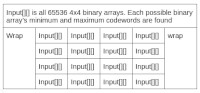
\includegraphics{inputGrid}\\
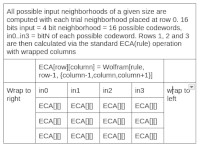
\includegraphics{ecaGrid}\\
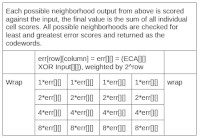
\includegraphics{errorGrid}\\
\end{center}

Having the minimizing and maximizing codewords for all inputs as above for a given ECA rule, it is applied to a 2D binary array or bitmap image as follows. For every (wrapped) (row,column) location in the input, the 4x4 local cell is the hexadecimal of that location and its right, down, and diagonal right-down neighbors $2^d$ away, $(row,column)..((row+2^d),(column+2^d))$  where d is depth of iteration. The value is replace with the respective minimizing or maximizing codewords. This comparing of neighbors of powers of 2 distance away is the same flow chart as the FFT and Fast Walsh Transforms in reverse with reminimizations instead of sums and/or products at every level of recursion. When the iteration's neighbor distance is $log2_{row}$ or $log_2(column)$, whichever is greater, every bit has influenced every other bit and has a unique distinct solution, detailed below. \\
\begin{center}
Below is a Fast Walsh-AlgorithmCode.Hadamard Example \cite{enwiki:1261916659}\\
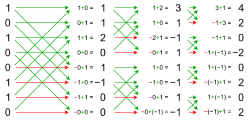
\includegraphics{FastWalshHadamard}\\
If you did the above with the powers of 2 in reverse order you would get this. \\
This the 1 dim version, and instead of a sum term it's a rehash.\\ 
Find the codewords of the codewords, twice as far apart each time.\\
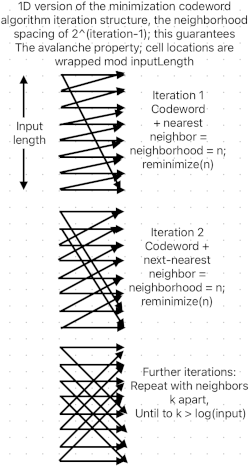
\includegraphics{AlgoStruct}\\
\end{center}

This transformation is perfectly invertible when using a complete minMax codeword rule set of 16. A single rule of the positive 8-tuple of the below is lossy, with an error rate of 3/8, however if the input is hashed as a set with every rule in the tuple, overlapping cells of every rule vote on their region of influence and the loss rate becomes 0. With a rectangular bitmap inverse, the overlapping codewords for all 16 of the rules in the subsets together make a weighted vote on the inverse of the algorithm. Each codeword is that location's best guess on its neighborhood and each location is part of at least 4 neighborhoods at each iteration, twice as far apart each time. The cell's best-gues output is weighted by its relative row or column and added to its location's tally of votes. At the end if the sum of the weighted votes is positive then it becomes 0, if it is negative it becomes 1. \\

\section{Hash properties}

Within the 256 ECA rules, there are 8 [0,15,51,85,170,204,240,255] that have the properties of unique codewords for any given input, every codeword occurs the same number of times with relatively even distribution of codewords across the 65536 neighborhoods in the truth table. 0 and 255 are included because in the 4 rows of the output matrix, 1 is neighborhood input and 3 are output, and so still produce an errorScore and therefore a unique solution. These properties apply to these rules with both errorScore minimization and errorScore maximization. \\

There is another overlapping subset of 8, [0,15,85,90,165,170,240,255] whose errorScore weight is $2^{row}$ rather than $2^{column}$. Again, the codewords are distributed perfectly evenly, there are unique solutions for every input, and has a minimizing and a maximizing codeword set. These lists share a few members with the XOR-additive list. \cite{xorAdditive}. Most properties apply to both with a few exceptions.\\

This algorithm can be used to make any sized hash. This hash is implemented to either hash-in-place so that the data stays the same size or as compression with the data size quartering each iteration. To implement any size output, first hash to the avalanche point as the fixed data size version, then as compression to the size desired and/or pad with zeroes. Rather than padding with zeroes one can use an inversion to expand the hash to a larger size, however inversion is more computationally expensive than compression. Another option is to hash to the avalanche point and take a subset of it. If using every minMax row-column codeword set, hash to desired size and then hash the hashes.\\

All 32 Wolfram codes in the 4 minMax row-column sets have a perfectly even distribution of codeword and every input has a unique solution. Each 0..15 codeword is used 4096 times, distributed relatively evenly across the 65536 possible binary 4x4 cells. The minMax row/column set as a whole has unique and distinct hash output with the hash-in-place version, so collisions do not happen. In the compression version individual rules' hashes are minimally collision resistant because the error weight difference means the bottom 2 rows or columns don't change the output much. This is greatly mitigated by using every codeword in the minMax row/column set due to the overlapping and transposed errorScore weights.\\

The hash-in-place version of the algorithm has a perfect inverse when working with complete sets of minMax row-column codewords and a roughly 2\% error when working with an individual rule's minMax codeword output. The compression version of the algorithm has a lossy inverse and again using complete rule sets reduces the error and every hash iteration increases the error. Individual rules have an average error of 6/16 per codeword.\\

Hashed input can be operated on with the row weighted rule set without the original input and without inverting it. Because these ECA rules in the 8-subset are linear; rules 15, 51, and 85 pass the left middle or right input bit with no other operation or dependency. Taking any 2 of 16 codeword-generated 4x4 cells and OR them together and reminimize, the result is the same as the original two codewords ANDed together.  This shift of logic operations within a hash is uniform within an ECA rule hash and extends to any depth of iteration; the hash algorithm transforms not only the input data but also the relative logic gate. For example if I want to retroactively apply a bitmask to a hashed image or IP address without the original image and without inversion, hash the bitmask and lookup the appropriate logic gate tranformation between the hashed image and the hashed bitmask. These operations only partially apply to the column weighted set, some of the rule-logic pairs have an operation transform and some do not, and no universal combination of gates has a complete set. \\

This algorithm displays some avalanche properties. The threshold for testing is when every pixel's RGB code has had an opportunity to influence every other pixel, or $log_2(imageWidth)$ or $log_2(imageHeight)$, whichever is greater. Experimentally changing small numbers of pixels and running the required number of iterations produce the property. What happens at that point is that triplets within a rule subset display a substantial number of changes on alternating iterations, and the sum between complementary rules is the total number of cells in the data. This shows that withing a complete codeword set, every single bit is affected by a change. On even iterations within the min codeword set, 15, 51, and 85 have many changes while 170, 204, and 240 don't, and the opposite on odd iterations. The same alternating happens with the column weighted errorScore set triplets to a lesser extent.\\

The 32 codewords for any 16 bit input display some symmetries generated by the same algorithm as the left-right-black-white symmetries of the ECA Wolfram code symmetry groups, applied to 4 bits. The left right symmetry is reversing the bit's place order and the black white symmetry is done by reversing the truth table and taking the complement and the left right black white is doing both operations. Applying this to the 4 bit codewords yields some symmetries but no two codeword sets have the same so there are no groups like the 88 independent sets in the ECA.\cite{Wolfram}\\

\section{Implementation, Testing, and Performance}

The algorithm is prototyped on 4-byte, 3-byte, and 2-byte RGB *.bmp bitmap files, including the first several images which come from a Linux screenshot then into *.bmp by GIMP. The program converts the image's raster in a rectangular hexadecimal array. Animated *.gif files are available at my website. You can see the areas of the image hashing 2 by 2 and slowly dissolving into avalanche territory that eventually just looks like noise everywhere. The current image was chosen because you can clearly see parts of the image doubling itself as the avalanche property slowly takes over. The code works with any size bitmap. Future work on the project would include other image formats as it is a color code hexadecimal conversion. \\

Testing\\


\begin{center}
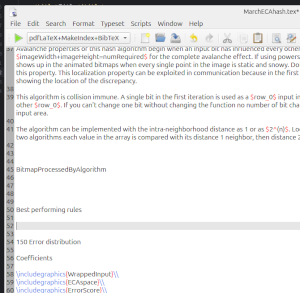
\includegraphics{testScreenshot}\\
Original Image\\
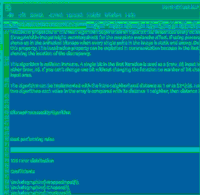
\includegraphics{processedDepth3}\\
Frame 3\\

\includegraphics{processedDepth6}\\
Frame 6\\
\end{center}

\section{Other rules, shapes, and sizes}

The weight in the errorScore sum can be $2^{row}$ or $2^{column}$, both produce the same set of 8 tuples with the unique solution and even distribution properties, though other ECA rules' properties don't necessarily carry over. This transposition and reflections across an axis may be enough to produce unique tuples without the loop, however checking this is ongoing.\\

The size of the input array can be easily be any power of 2 squared. Within this prototype project, calculation of Wolfram code lengths of $2^{16}$ using all 4x4 binary grids are acceptable, lengths of $2^{64}$ using 8x8 grids would be challenging at this point. At size 8 there are $2^8=256$ possible codewords, which means that while you can't calculate the whole truth table at once you can calculate the codewords individually on the spot. The 8 tuple's uniqueness and distribution properties probably apply at larger sizes, it may not; it is only exhaustively tested for size 4 and size 8 is only randomly spot-checked. The internal hash logic transforms can still be easily calculated for size 8 because you only have to work with codewords rather than the entire set of inputs. Sizes other than 4 and 8 are not considered here.\\

Out of the other 0-255 ECA rules, some do better than these particular 8 at lossy compression, losing only 3/16 bits instead of 6/16 bits with these 8. In particular the Pascal rules 90, 165, 102, 153, 105, 150 rank near the top, connected to several these 8 via the property of XOR-additiveness (cite wolfram atlas). However none outside of these 8 have unique solutions or even distributions in either row or column weighted, maxxed or minned.\\

\section{Rule 150}

If while running this algorithm for rule 150 you produce a heat map of the errors in reconstructing the lossy compression, you get this. To seven binary digits, five past the decimal place, Phi and Pi show up in these ratios. Seven binary digits is a 2\% error rate. Seven digits is enough for an ASCII operation. Precision to seven decimal places shows up here and in reconstructing the 8-tuples above. If you label a five point star and proceed backwards starting at 0, you get \{3,1,4,2,0\} which is roughly the same seven digit precision. Some of those mentioned here are seven binary digits some are accurate to nine. While seven digits by itself is not impressive, 7 digits across three constants is notable.\\

\noindent rule 150\\

\noindent minErrorMap\\
29482 29482 29476 29464 \\
30940 30904 30958 30958 \\
17486 17486 17516 17576 \\
5532 5592 5502 5502 \\

\noindent minProportions[][]\\
1.0000 0.9527 1.6828 5.3283 \\
1.0497 1.0000 1.7664 5.5929 \\
0.5942 0.5661 1.0000 3.1663 \\
0.1877 0.1788 0.3158 1.0000 \\
2.621312044429018\\

\noindent a = row2 / row 3 = 3.166305133767173\\
a = (row2 / row 3) - PI = 0.024712480177379703\\
accurate to the binary -5 place\\

\noindent b = row1 / row 0 = 1.0496675261229476\\
b = (row1 / row 1) - (PI/3) = 0.002469974926349927\\
accurate to the binary -9 place\\

\noindent c = (row0+row1)/(row2+row3) = 2.621312044429018\\
c = (row0+row1)/(row2+row3) - PhiSquared = 0.003278055679122982\\
accurate to the binary -8 place\\

\noindent Throw in the 1's and 2's place makes for 7, 11, and 10 accurate digits\\
If you compare that accuracy to the method of computing pi by the edges of increasing numbers of triangles\\
it takes dividing 2Pi into 32 triangles to get 7 digits. If takes 32 iterations of the Wallis product\\

\bibliographystyle{plain}
\bibliography{HashBib.bib}

\end{document}